\chapter{Introduction}

\section{Motivation}
Machine learning (ML) is a big research area in computer science and especially here at TU Darmstadt. Many groups in the computer science departments do research on ML either directly or indirectly by using it to achieve some other goal/knowledge (e.g. for image recognition or natural language processing). Research on computer languages concerning problems specific to ML could facilitate the implementation of ML applications for many use cases. Because of this the Software Technology Group at TU Darmstadt also wants to focus more on ML. Gradient descent and therefore differentiable programming builds the base of ML which makes it the perfect starting point for a newly found focus on ML. Having an overview of possible implementations would make it possible to decide which implementation is best suited to design a ML library, algorithm or even (domain specific) language around. 

Our goal for this work is to produce such an overview by implementing differentiation in multiple ways. These will be partly based on other's work which we (re-)implement and adjust to fit a similar implementation style so that we can easily compare all implementations. Furthermore we will extend those implementations with new functionalities, change them from the ground up or implement our own designs from scratch. Secondarily we will try to find use cases of the new language features introduced in Scala 3 to get an idea if this language has potential to aid implementing ML tasks.

\section{Overview}
Firstly we provide an overview over our work. We start off with implementing the normal well-known forward mode differentiation in \refsec{sec:forwardMode}. For this we first give a quick view on how to use a naive but unorthodox way to implement it using macros to replace code in \refsec{sec:macros}. After that we introduce the more common dual numbers in \refsec{sec:forwardDualNumbers} which will be a key ingredient also for later (reverse mode) implementations. The next implementation gets more experimental again. In \refsec{sec:matchTypes} we use the newly introduced match types and value types of Scala 3 to implement a symbolic differentiation-like way to produce a derivative completely at type level in compile time.

The main focus of this work is definitely \refsec{sec:reverseMode} because reverse mode is much more interesting for ML tasks than forward mode. Here we begin by introducing the mathematical background of reverse mode by doing it once ``by hand''. As using mutation and non-functional programming usually leads to an arguably more straight forward implementation we for now continue without restricting us to functional programming in \refsec{sec:mutation}. We introduce continuation passing style (CPS) which at first seems like unnecessary overhead and in itself may be hard to wrap your head around at first. However it pays off when it elegantly demystifies how to implement reverse mode differentiation in \refsec{sec:cps}. Using a tape to store operations on in \refsec{sec:tape} is also a valid way to implement reverse mode in a similar way to CPS. From there we continue to wrap CPS into a monad in \refsec{sec:monadCPS} to facilitate usage of CPS from the client side. We finish the mutation section by combining the monad and tape idea in \refsec{sec:monadAndTape}.

For the more puristic oriented in \refsec{sec:noMutation} we translate the CPS and monad implementations in \refsec{sec:functionalCps} and \refsec{sec:functionalMonad} respectively into a design which does use an accumulator to map expressions to their adjoints instead of mutation. The last implementation \refsec{sec:chad} is fully functional and doesn't even need a unique ID per expression which consequently means it only needs value equality to function. On top of that it is easily comprehensible because it comes without much overhead or complicated abstractions.

\todocite{section}
In the end we will compare the runtime performance of each implementation.

\section{External Work}
In conclusion we want to give a quick overview over which sections are based on which external work. \emph{CHAD: Combinatory Homomorphic Automatic Differentiation} \cite{chad} is the base for \refsec{sec:chad}. \emph{Demystifying Differentiable Programming: Shift/Reset the Penultimate Backpropagator} \cite{lantern} has a running example of a function which is differentiated. This function is also used throughout our work as a running example. Furthermore we based \refsec{sec:forwardDualNumbers}, \refsec{sec:cps}, \refsec{sec:tape} and \refsec{sec:functionalCps} directly on their work. Other reverse mode sections, namely \refsec{sec:monadCPS}, \refsec{sec:monadAndTape} and \refsec{sec:functionalMonad}, are mainly based on our own work but do refer to or build on concepts introduced in the previously mentioned sections and therefore are indirectly based on the work of Fei Wang et al. 



















% Hello
% For this work I need to cite \cite{abc12}. And \cite{tudapub}

% \section{bla}

% \subsection{blubb}

% Have a look at figure \ref{uml_example} to see how including images works.

% \begin{figure}
%     \centering
%     remember to include a path relative to your root .tex file
%     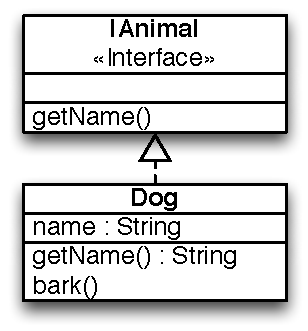
\includegraphics[width=4cm]{images/uml}
%     \caption{Sample UML Diagram}
%     \label{uml_example}
% \end{figure}

% \subsection{blubb 2}

% Avoid single subsections! Each ``parent'' has to have at least two ``childs''

% \section{bla 2}
